\chapter{Implementação}
\label{implementacao}

\section{Stack Tecnológico}
\label{sec:stack-tecnologico}

A camada de coleta e transformação foi implementada em \textit{Python} e \textit{Tableau Prep Builder}, aproveitando o ecossistema científico da linguagem para a manipulação de séries temporais financeiras. A biblioteca \textit{yfinance} foi adotada como interface programática com o provedor público de dados financeiros, enquanto o \textit{Tableau} concentrou as operações de criação de chaves, junções entre tabelas e limpeza geral dos dados.

A camada de armazenamento é sustentada pelo \textit{PostgreSQL}, escolhido por seu suporte robusto a tipos numéricos de precisão dupla, por sua maturidade no tratamento de junções entre tabelas volumosas e por suas capacidades analíticas via \textit{Common Table Expressions} e funções de janela, recursos amplamente utilizados nas consultas que alimentam o painel.

A camada de aplicação foi construída em \textit{Node.js} sobre o \textit{framework Express}, organizada no padrão arquitetural \textit{controller}, \textit{repository} e \textit{service}. O controlador recebe e valida os parâmetros das requisições, o repositório concentra a lógica SQL analítica, e o serviço auxiliar carrega o histórico do S\&P 500 em memória para servir como \textit{benchmark} sob demanda. A API expõe \textit{endpoints REST} que respondem em JSON e isolam o \textit{frontend} de qualquer dependência direta com o banco.

A camada de visualização foi desenvolvida em \textit{React}, com gráficos renderizados pela biblioteca \textit{Recharts}. A escolha do \textit{Recharts} se deveu à sua integração nativa com o paradigma declarativo do \textit{React} e à flexibilidade na composição de eixos, séries e indicadores customizados, necessária para a apresentação simultânea do índice sintético, do \textit{benchmark} e dos modificadores de risco. O stack tecnológico completo deste trabalho pode ser verificado no Quadro \ref{tab:stack}

\begin{table}[ht]
\centering
\caption{Componentes da stack tecnológica do ambiente analítico}
\label{tab:stack}
\begin{tabular}{|p{4.5cm}|p{4.5cm}|p{5cm}|}
\hline
\textbf{Camada} & \textbf{Tecnologia} & \textbf{Função} \\
\hline
Coleta e transformação & \textit{Python}, \textit{pandas}, \textit{yfinance}, \textit{Tableau} & Extração, tratamento e cálculo de risco \\
Armazenamento & PostgreSQL & Data Warehouse dimensional \\
Aplicação & Node.js, Express & API REST analítica \\
Visualização & React, Recharts & Painel interativo \\
\hline
\end{tabular}
\fonte{Elaborado pelos autores.}
\end{table}

\section{Conversão do Modelo Lógico para o Modelo Físico}
\label{sec:arquitetura-dw}

O modelo lógico apresentado na Seção \ref{sec:modelagem-dimensional} foi convertido em modelo físico e materializado no \textit{PostgreSQL} por meio de instruções SQL, sob o banco \texttt{tcc\_indices}, preservando integralmente a topologia de esquema estrela definida no projeto. A conversão para o modelo físico envolveu três decisões atreladas ao SGBD escolhido: a adoção de tipos numéricos de precisão dupla para os atributos monetários e estatísticos, a nomeação padronizada de tabelas e colunas com prefixos identificadores de dimensão (\texttt{dim\_}) e fato (\texttt{fato\_}), e a definição explícita das restrições de integridade referencial entre as chaves estrangeiras das tabelas fato e as chaves primárias das tabelas dimensão.

\section{Planejamento das Análises}
\label{sec:planejamentoconsultas}

Antes da implementação de qualquer consulta SQL ou componente visual, conduziu-se uma etapa de planejamento dedicada a delimitar o que o ambiente analítico deveria ser capaz de responder. Ao antecipar o desenho das perguntas em relação à escrita do código, garantimos que cada consulta posteriormente implementada tivesse uma motivação analítica clara, vinculada aos conceitos discutidos no Capítulo \ref{fundamentacao} e à métrica de Risco Modificado descrita no Capítulo \ref{metodologia}. E orientamos a construção da camada visual a partir do conteúdo informacional, e não o contrário, evitando que a escolha de gráficos disponíveis na biblioteca de visualização condicionasse o tipo de análise oferecida ao usuário.

O ponto de partida do planejamento foi a definição do usuário hipotético do protótipo: um investidor que, a partir de seu perfil de tolerância à perda no referencial de \citeonline{assaf_neto_mercado_2022}, deseja explorar o mercado norte-americano de forma estruturada. A partir dessa figura, foram elencadas as questões que esse usuário tipicamente formularia ao confrontar a base de dados, organizadas em três blocos temáticos: comportamento agregado do mercado por setor, comportamento condicionado às faixas de risco e construção de uma carteira individual. Cada bloco gerou um conjunto de perguntas em linguagem natural, que serviram de especificação direta para as consultas SQL implementadas e para as visualizações correspondentes no \textit{dashboard}.

No bloco de comportamento agregado por setor, as perguntas formuladas foram:

\begin{enumerate}
    \item Como evoluiu o preço médio das ações de cada setor ao longo do recorte temporal selecionado?
    \item Qual a volatilidade anualizada dos retornos de cada setor no período analisado?
    \item Existe sazonalidade no retorno médio mensal dos setores ao longo do ano com base no período selecionado?
    \item Qual o grau de correlação entre as séries semanais de preço agregado dos diferentes setores, e quais pares apresentam comportamento mais independente?
\end{enumerate}

No bloco de comportamento condicionado às faixas de risco, as perguntas foram:

\begin{enumerate}
    \item O retorno anualizado das ações cresce monotonicamente com o aumento da faixa de risco, conforme previsto pela teoria tradicional, ou observa-se o paradoxo de baixa volatilidade?
    \item Qual a maior retração de pico a vale (\textit{Maximum Drawdown}) observada em cada faixa de risco frente ao mesmo evento de mercado?
    \item Qual setor concentra maior exposição sistêmica ao risco, medida pelo \textit{Z-score} agregado de seus ativos?
    \item Como se compara a trajetória cumulativa de carteiras agrupadas por faixa de risco frente à trajetória do S\&P 500 no mesmo período?
\end{enumerate}

No bloco de construção de carteira individual, as perguntas foram:

\begin{enumerate}
    \item Dados os mesmos filtros, quais ativos apresentam a maior pontuação composta de qualidade, e qual o peso relativo que cada um deveria receber em uma alocação?
    \item Considerando o conjunto de ativos selecionado pelo usuário e os pesos derivados de sua pontuação, como teria evoluído essa carteira customizada em comparação com o S\&P 500 no recorte temporal definido?
    \item Dados os filtros de país, setor, indústria e faixa de risco escolhidos pelo usuário, quais ações compõem o universo selecionado, qual o perfil atual de cada uma e como seu risco estatístico se compara ao Risco Modificado obtido após a incorporação dos indicadores com pesos $\alpha$ configuráveis?
\end{enumerate}

Cada uma dessas perguntas foi mapeada de forma direta para um \textit{endpoint} da API \textit{REST} e para uma aba do painel, preservando a rastreabilidade entre a intenção analítica original e a sua materialização técnica. O Quadro \ref{tab:mapeamentoconsultas} descreve esse mapeamento.

\begin{table}[h]
\centering
\caption{Mapeamento entre as perguntas em linguagem natural, os \textit{endpoints} da API e as abas do painel.}
\label{tab:mapeamentoconsultas}
\begin{tabular}{|p{5.5cm}|p{4cm}|p{4cm}|}
\hline
\textbf{Pergunta} & \textbf{Endpoint} & \textbf{Aba do painel} \\ \hline
Evolução setorial em base comum & \texttt{/indice} & Performance \\ \hline
Volatilidade anualizada por setor & \texttt{/volatilidade} & Volatilidade \\ \hline
Sazonalidade do retorno mensal & \texttt{/sazonalidade} & Sazonalidade \\ \hline
Correlação entre setores & \texttt{/correlacao} & Correlação \\ \hline
Retorno por faixa de risco & \texttt{/anomalia-risco} & Anomalia Risco \\ \hline
\textit{Maximum Drawdown} por faixa & \texttt{/estresse-risco} & Teste de Estresse \\ \hline
Exposição sistêmica setorial & \texttt{/exposicao-setorial} & Exposição Setorial \\ \hline
Evolução de carteiras por risco & \texttt{/evolucao-risco} & Evolução por Risco \\ \hline
Alocação \textit{smart beta} por setor & \texttt{/mapa-mercado} & Mapa de Mercado \\ \hline
Backtest de carteira customizada & \texttt{/indice-customizado} & Mapa de Mercado \\ \hline
Listagem detalhada com Risco Modificado por ativo & \texttt{/listagem-acoes} & Listagem de Ações \\ \hline
\end{tabular}
\end{table}

\section{Construção do \textit{Dashboard}}
\label{sec:construcao-dashboard}

A camada de visualização do trabalho foi implementada em \textit{React}, consumindo os \textit{endpoints} descritos na seção \ref{sec:planejamentoconsultas} e renderizando os resultados por meio da biblioteca \textit{Recharts}. O componente \texttt{App.jsx} centraliza o estado dos filtros e dispara as requisições à API; o componente \texttt{FiltrosCascata.jsx} encapsula os controles de seleção; o componente \texttt{PainelVisualizacao.jsx} concentra a lógica de cada aba analítica. A organização em três componentes principais separa a orquestração de estado, a captura de parâmetros do usuário e a renderização gráfica, permitindo que cada aba reaproveite o mesmo conjunto de filtros sem duplicação de código.\ref{fig:capaCompleto}

\begin{figure}[htb]
   \centering
   \caption{Tela inicial do ambiente analítico.}
   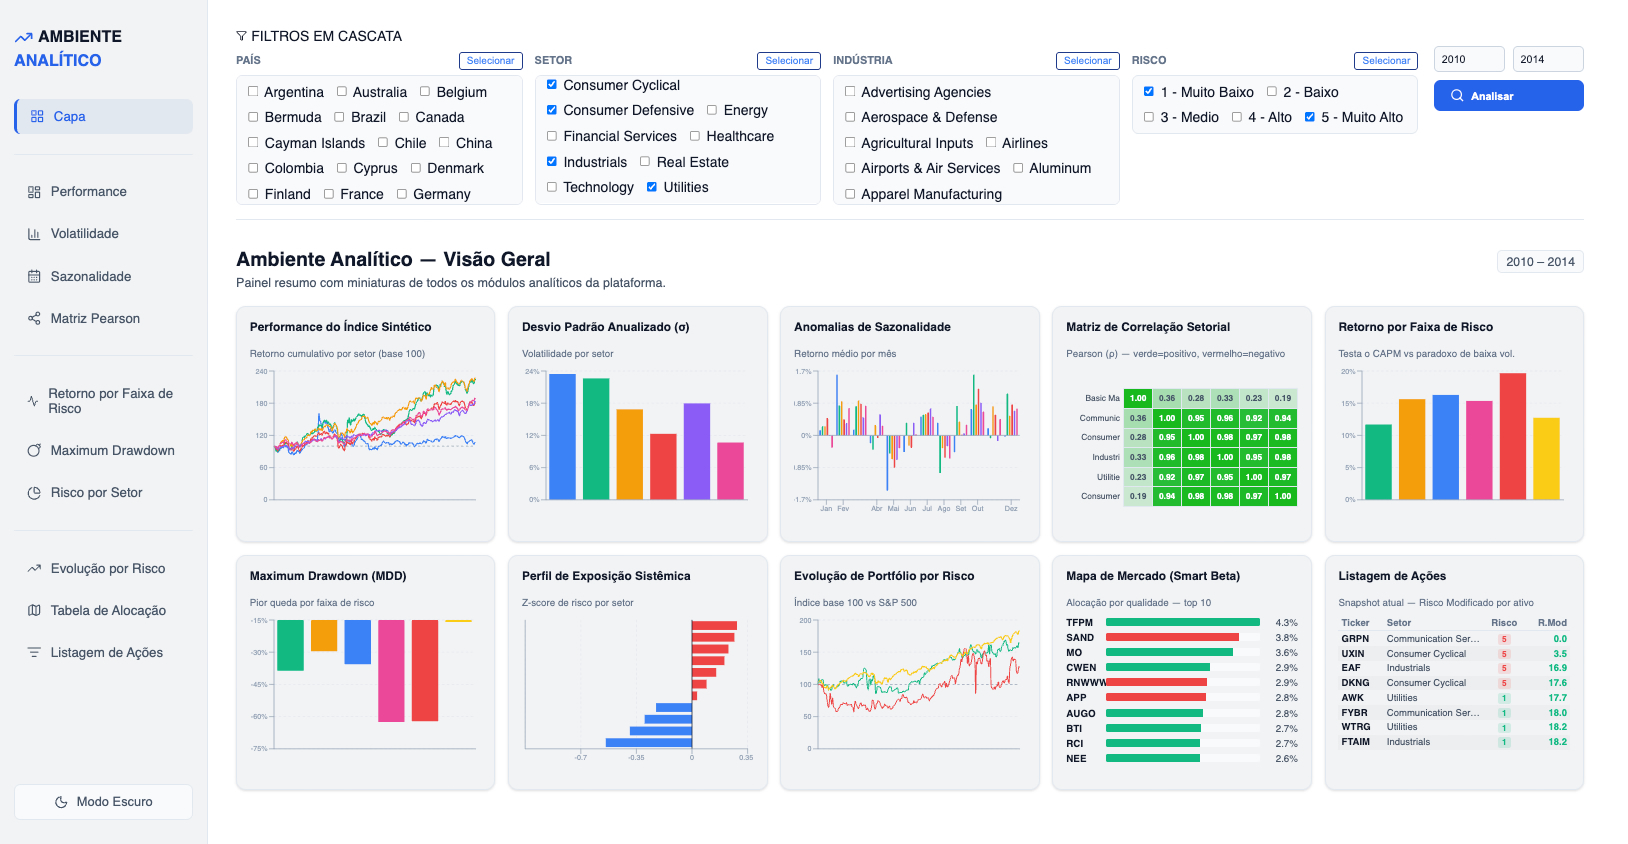
\includegraphics[width=\textwidth]{figuras/capaCompleto.jpg}
   \label{fig:capaCompleto}
   \fonte{Elaborado pelos autores.}
\end{figure}

Grande parte da agilidade obtida nessa etapa decorreu diretamente das camadas construídas anteriormente. A modelagem dimensional em esquema estrela, apresentada na Seção \ref{sec:modelagem-dimensional} e materializada no modelo físico descrito na Seção \ref{sec:arquitetura-dw}, forneceu ao painel uma estrutura de consulta previsível: os filtros em cascata de país, setor, indústria e faixa de risco correspondem de forma quase direta aos atributos já normalizados nas tabelas dimensão, o que dispensou qualquer reorganização dos dados no \textit{frontend}. De modo análogo, a etapa de coleta e transformação já havia calculado os indicadores de risco e classificado cada ativo em sua faixa, de forma que o painel não precisou reproduzir nenhuma lógica estatística em tempo de execução, limitando-se a requisitar recortes de valores previamente calculados. O esforço de implementação da camada visual concentrou-se, portanto, na composição dos gráficos e na interatividade dos filtros, e não no tratamento ou no enriquecimento dos dados, tarefas já resolvidas nas camadas de modelagem e de transformação.

A construção do \textit{dashboard} foi feita com base nas ideias apresentadas no início do projeto. A primeira delas é que o trabalho deve ser parametrizável por janela temporal e por recortes setoriais. A segunda estabelece a coexistência de duas perspectivas de análise, uma histórica e outra de cenário atual, justificada pela disponibilidade desigual dos dados institucionais em relação às séries de cotação. A terceira impõe que toda comparação entre a carteira analisada e o \textit{benchmark} (S\&P500) sejam apresentadas em um único gráfico e com a mesma escala, evitando interpretações enviesadas.

\subsection{Protótipo Dinâmico e Detalhamento por Setor e Faixa de Risco}
\label{subsec:prototipo-dinamico}

O \textit{dashboard} foi tratado como prototipagem de um ambiente analítico, e não como produto final destinado ao mercado. Essa caracterização define o escopo da implementação visual e direciona o esforço para a interatividade dos filtros, e não para a robustez de uma aplicação em produção.

\begin{figure}[htb]
   \centering
   \caption{Seção de filtros do \textit{dashboard}.}
   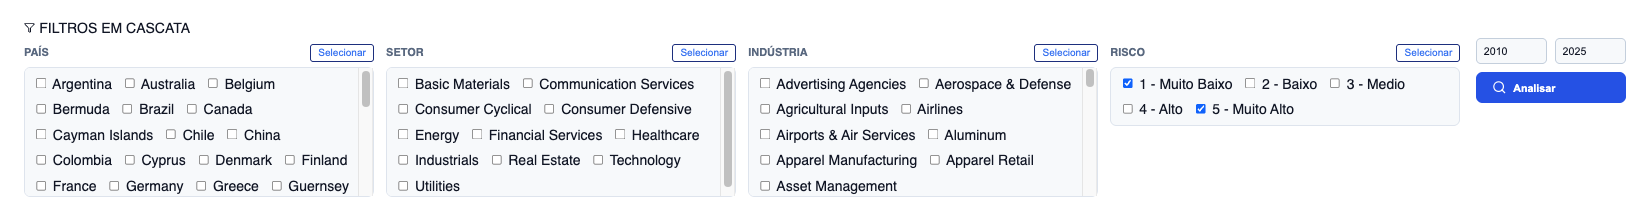
\includegraphics[width=\textwidth]{figuras/filtros.png}
   \label{fig:listagem-acoes}
   \fonte{Elaborado pelos autores.}
\end{figure}

A seleção de país restringe as opções de setor, que por sua vez restringem as opções de indústria, que finalmente são cruzadas com a faixa de risco. Em paralelo, dois campos numéricos definem o ano inicial e o ano final da janela de análise, com limites entre 2010 e 2025. Toda alteração nesses controles dispara, via efeito colateral do \textit{React}, uma nova chamada aos \textit{endpoints} ativos na aba em uso, atualizando os gráficos em tempo de execução. Essa arquitetura atende à recomendação de que o \textit{dashboard} não fosse estático, permitindo ao usuário alternar livremente entre recortes temporais de qualquer intervalo de anos sem necessidade de reexecutar consultas no banco.

A interatividade dos filtros é o que viabiliza, na prática, o detalhamento. Partindo de uma visualização por setor, como o índice sintético da aba Performance ou as barras da aba Exposição Setorial, o usuário pode estreitar progressivamente o universo até identificar quais empresas integram determinado setor e determinada faixa de risco. A aba Listagem de Ações encerra esse percurso de detalhamento, apresentando o conjunto resultante em uma tabela com colunas de identificação, risco normalizado, risco modificado e indicadores. A combinação entre as abas agregadas e a Listagem materializa o que a literatura de \textit{business intelligence} denomina \textit{drill-down}, conforme apresentado por \citeonline{kimball_data_2013}, oferecendo ao usuário trajetórias coerentes entre a visão geral e a visão ativo a ativo. As faixas de risco constituem a quarta dimensão do filtro em cascata e diferem das demais por não derivarem de um atributo cadastral da ação, mas de um cálculo estatístico prévio.

\subsection{Visão Histórica e Visão de Cenário Atual}
\label{subsec:duas-perspectivas}

O \textit{dashboard} foi organizado tendo em mente a perspectiva histórica, que reúne as abas que exploram as séries temporais densas, isto é, Performance, Volatilidade, Sazonalidade, Correlação, Anomalia de Risco, Teste de Estresse e Evolução por Risco. Mas também a perspectiva de cenário atual que concentra-se nas abas que dependem dos indicadores, isto é, Tabela de Alocação e Listagem de Ações. Nessas duas abas, os modificadores operam sobre o último registro disponível de cada ação, essa escolha decorre de uma limitação no fornecimento de dados da API, que disponibiliza os indicadores apenas como um recorte pontual, e não como série histórica. A Figura\ref{fig:alocacaoCompleto} mostra os modificadores utilizados no calculo de risco aplicados sobre o recorte temporal.

\begin{figure}[htb]
   \centering
   \caption{Aba de alocação, representativa da perspectiva de cenário atual, com o \textit{backtest} da carteira customizada frente ao S\&P 500.}
   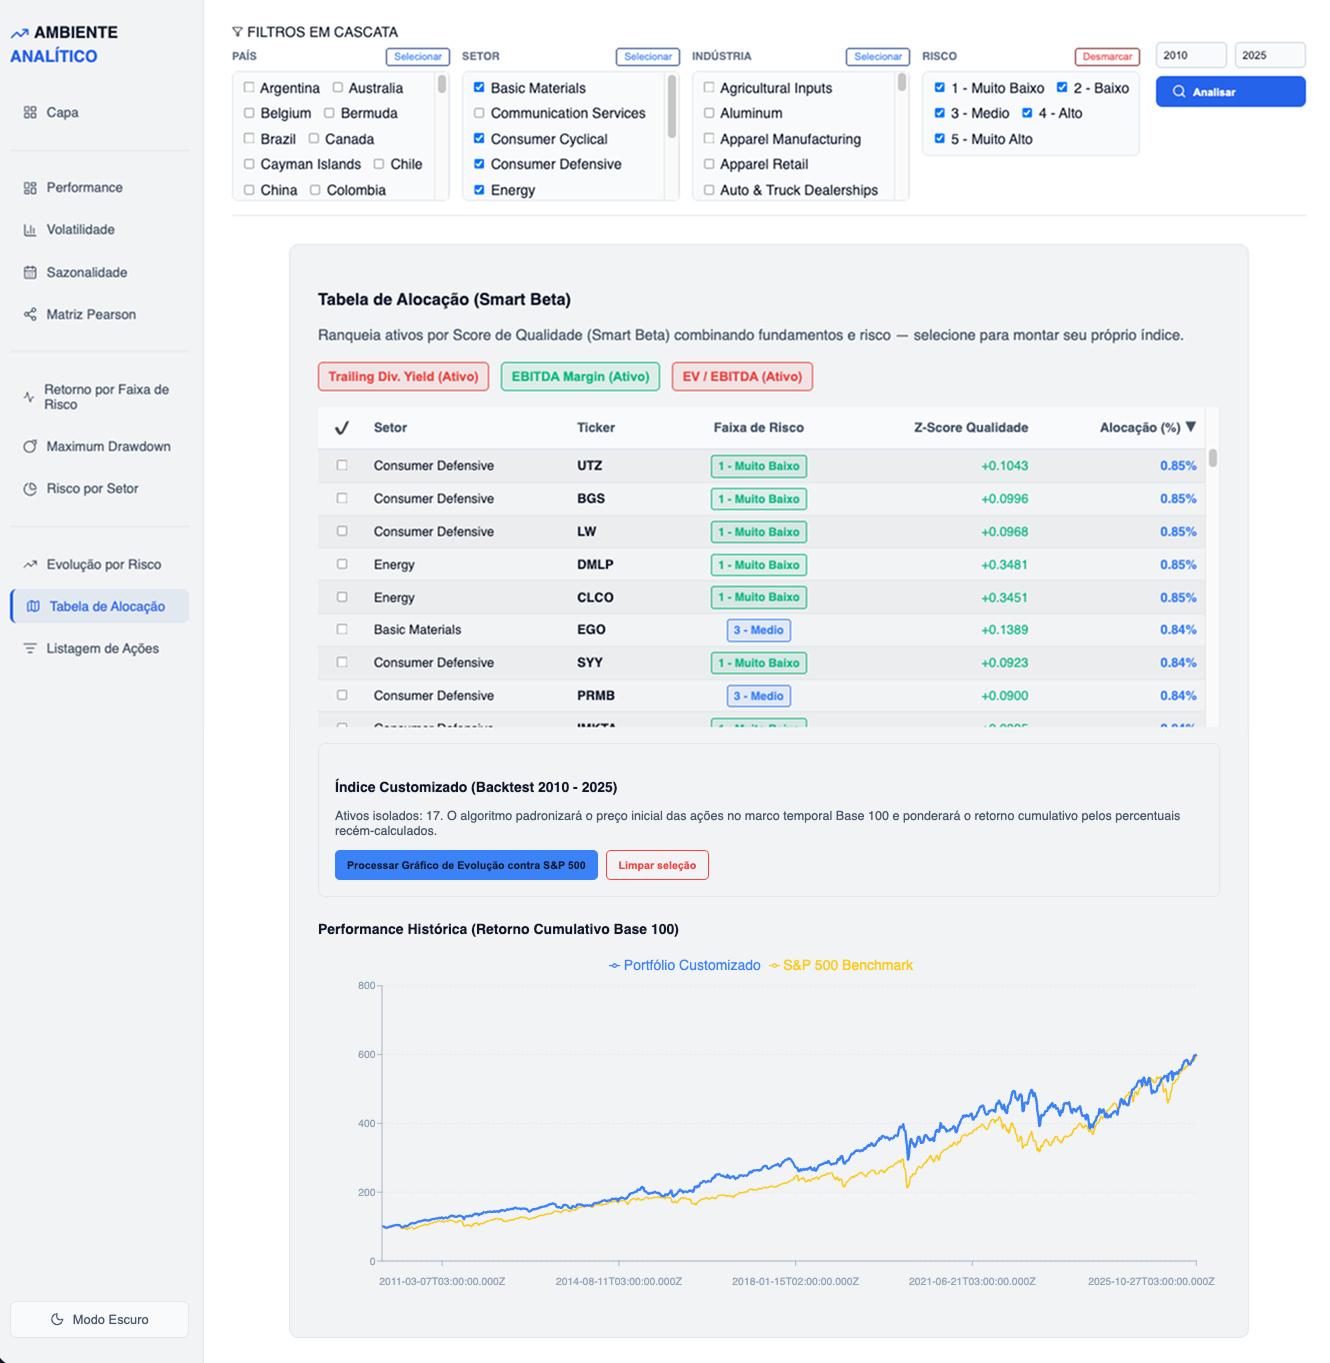
\includegraphics[width=\textwidth]{figuras/alocacaoCompleto.png}
   \label{fig:alocacaoCompleto}
   \fonte{Elaborado pelos autores.}
\end{figure}

\subsection{Consulta Paramétrica de Ações}
\label{subsec:consulta-parametrica}

Dentro da perspectiva de cenário atual introduzida na subseção anterior, a aba Listagem de Ações ocupa uma posição particular: é a única do \textit{dashboard} em que o usuário não apenas filtra o conjunto de resultados, mas também intervém diretamente na fórmula que produz o próprio indicador exibido. Enquanto as demais abas oferecem parâmetros que apenas recortam dados pré-calculados, essa aba, visível na figura \ref{fig:listagemCompleto}, expõe ao usuário os coeficientes internos do Risco Modificado, permitindo que a mesma base de ativos seja reavaliada sob diferentes configurações do modelo sem qualquer intervenção no código.

\begin{figure}[htb]
   \centering
   \caption{Aba Listagem de Ações, com os pesos $\alpha$ da fórmula do Risco Modificado editáveis pelo usuário.}
   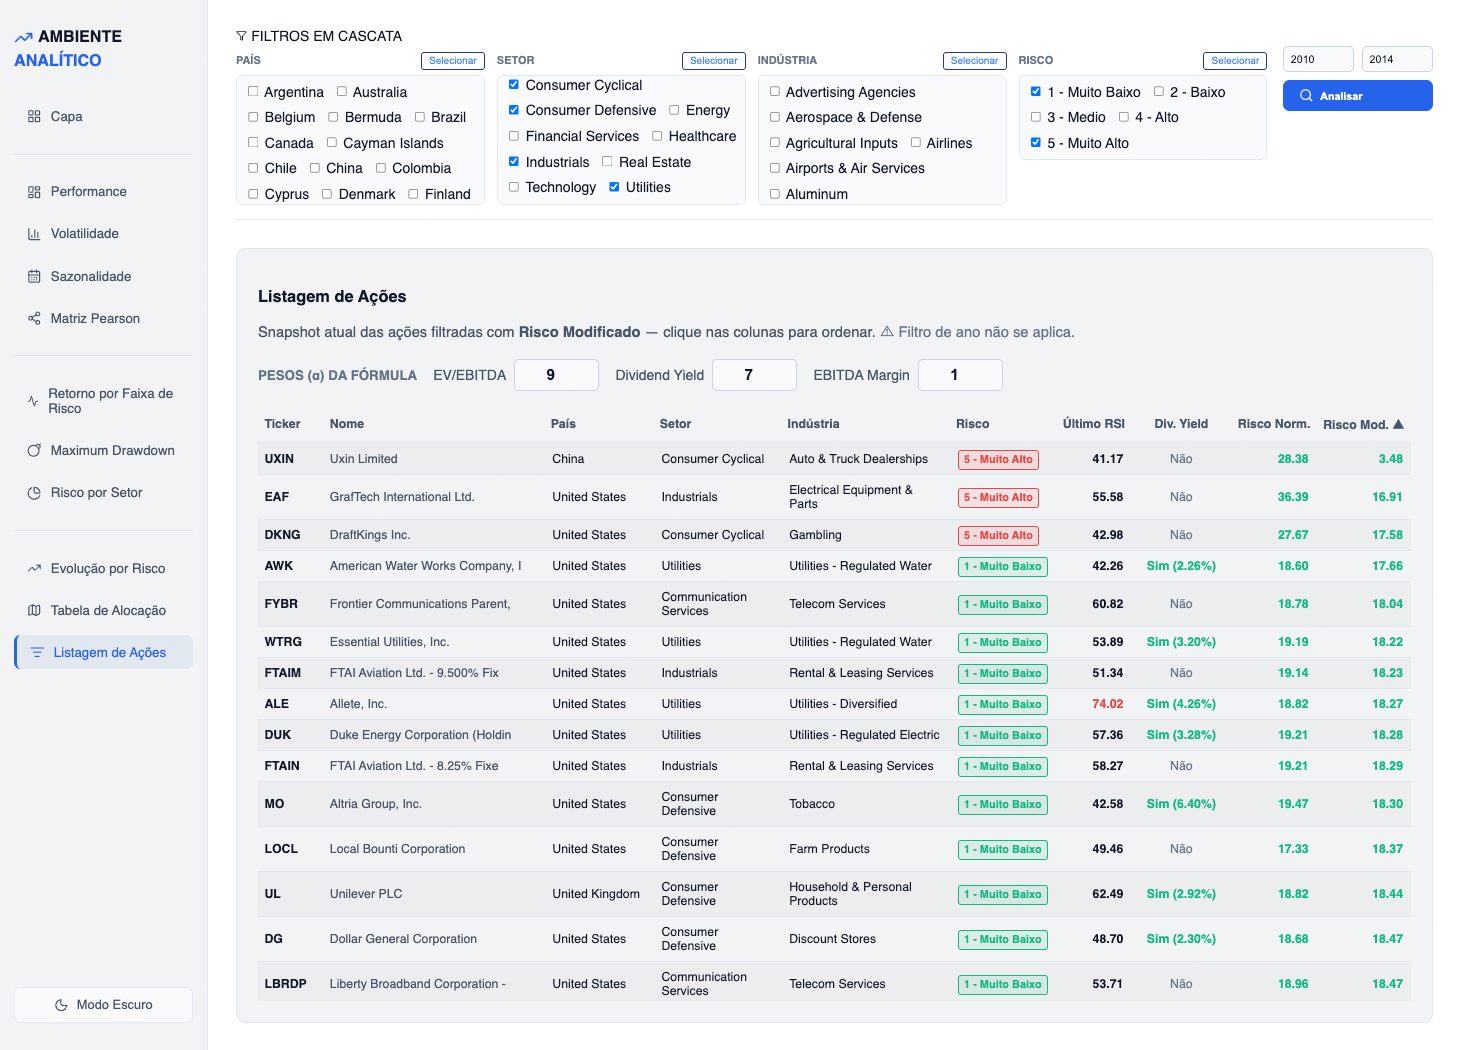
\includegraphics[width=\textwidth]{figuras/listagemCompleto.jpg}
   \label{fig:listagemCompleto}
   \fonte{Elaborado pelos autores.}
\end{figure}

Essa combinação transforma a aba em um instrumento de experimentação: zerando um peso, sua contribuição à fórmula desaparece; isolando um único peso, é possível medir o efeito exclusivo de um modificador sobre o conjunto de ações retornado; e combinando os três pesos nos valores padrão, obtém-se a configuração final proposta pelo modelo. O usuário pode, assim, formular perguntas do tipo "quais ações de determinado setor permanecem em faixa de risco muito baixa mesmo após a aplicação de todos os modificadores", e obter a resposta diretamente na tabela, sem necessidade de reescrever consultas SQL ou de alternar entre ferramentas distintas.